%--------------------------------------------------------------
%--------------------------------------------------------------
% Section 4 :  MPTK for Mac OS
%--------------------------------------------------------------
%--------------------------------------------------------------
\chapter{MPTK for Mac OS \label{MptkForMac}}

%--------------------------------------------------------------
% Section 4.1 : Downloading MPTK
%--------------------------------------------------------------
\section{Downloading MPTK}

The latest version of MPTK is available at (https://gforge.inria.fr/frs/?group\_id=36). Depending on the processor architecture 
of your computer, you will have to download either the 32 bits package or the 64 bits package:
\begin{my_itemize}
	\item For Mac 32 bits : ``MPTK-binary-v.v.v-i386-Mac.exe''
	\item For Mac 64 bits : `MPTK-binary-v.v.v-x86\_64-Mac.exe''
\end{my_itemize}

\noindent \emph{\underline{Hint :} To find the processor architecture of your computer :}
\begin{my_itemize}
	\item \emph{Open a terminal command and use the following command : \textbf{uname -m}}
	\begin{my_itemize}
		\item \emph{If the answer is ``i386'' then your OS is 32 bits}
		\item \emph{If the answer is ``x86\_64'' then your OS is 64 bits}
	\end{my_itemize}
\end{my_itemize}

%--------------------------------------------------------------
% Section 4.2 : Obtaining additional required packages
%--------------------------------------------------------------
\section{Obtaining additional required packages}

Two additional packages are needed. Their installation require administrator privileges on the machine. 
The ``sudo''  command may ask you to input administrator password :
\begin{my_itemize}
	\item Libsndfile (tested with version 1.0.23) pre compiled library
	\item FFTW (tested with version 3.2.2) pre compiled library
        \item Optional, but required to enable the Python wrapper pyMPTK:
        \begin{my_itemize}
                       \item Python (tested with version 2.7)
                       \item NumPy (tested with version 1.5)
                       \item Matplotlib (tested with version 1.0)
        \end{my_itemize}
\end{my_itemize}

\noindent You can see below some examples about how to download those libraries using terminal: 

\vspace{0.3 cm}

\begin{center}
	\begin{tabular}{|c|}
		\hline
		\rowcolor[gray]{0.35} \textcolor{white}{\emph{Mac}} \\
		\hline \hline
			\begin{tiny}
				\emph{sudo /opt/local/bin/port install libsndfile +universal}
			\end{tiny} \\
			\begin{tiny}
				\emph{sudo /opt/local/bin/port install fftw-3 +universal}
			\end{tiny} \\
		\hline
	\end{tabular}
\end{center}

\noindent \emph{\underline{Hint :} We suggest to use the ``port'' command from MacPorts because the command 
``+universal'' allows to retrieve libraries which are compatible with both system architectures (32 bits and 64 bits). 
The package is available at http://www.macports.org/install.php}

For the Python requirements, note that the core Python programming language is pre-installed on all Macs.
However, there are different ways to get a full Python install with the numerical and plotting libraries included,
We recommend you consult the information at \texttt{http://new.scipy.org/download.html} -- some users have had good
experiences with the Enthought distribution, some using Macports (as above) or Homebrew.


%--------------------------------------------------------------
% Section 4.3 : Installing MPTK
%--------------------------------------------------------------
\section{Installing MPTK}

When double clicking the executable \textbf{``MPTK-binary-v.v.v.-(i386/x86\_64)-Mac.dmg''}:
\begin{enumerate}
	\item Accept the terms of the licence agreements
	\item Accept the path folder where to install MPTK
	\begin{my_itemize}
		\item The default and unique folder is : ``/usr/local/''
	\end{my_itemize}
	\item Finish the installation
\end{enumerate}

\begin{figure}[H]
	\begin{minipage}[t]{.4\linewidth}
   	 	\begin{center}
			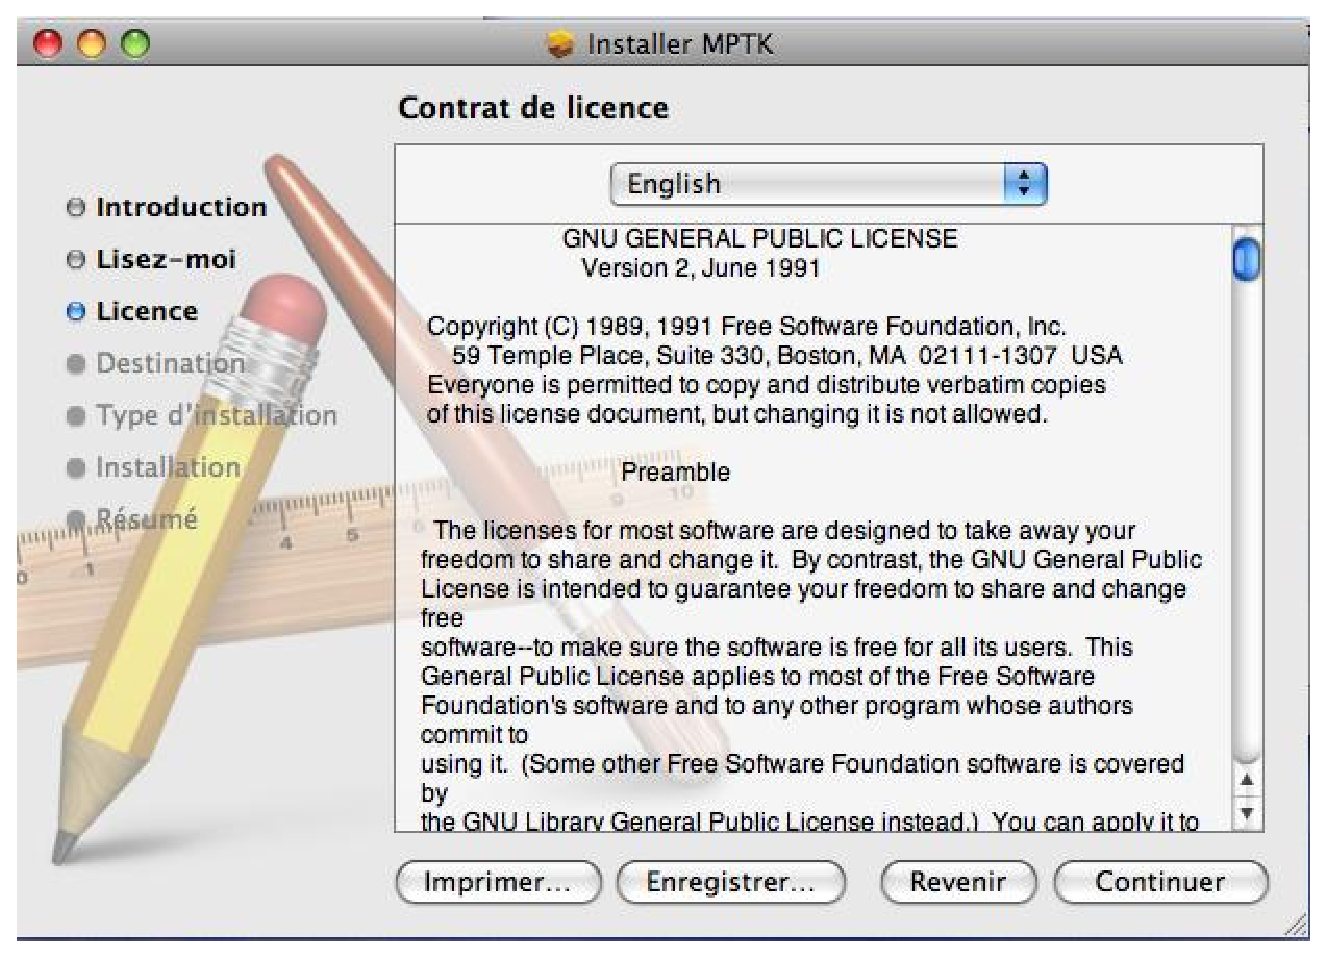
\includegraphics[width = 7cm, height=5cm]{Images/MacLicence.eps}
			\textit{\caption{\label{MacLicence} Licence agreement}}
		\end{center}
	\end{minipage}
	\hfill
	\begin{minipage}[t]{.4\linewidth}
		\begin{center}
			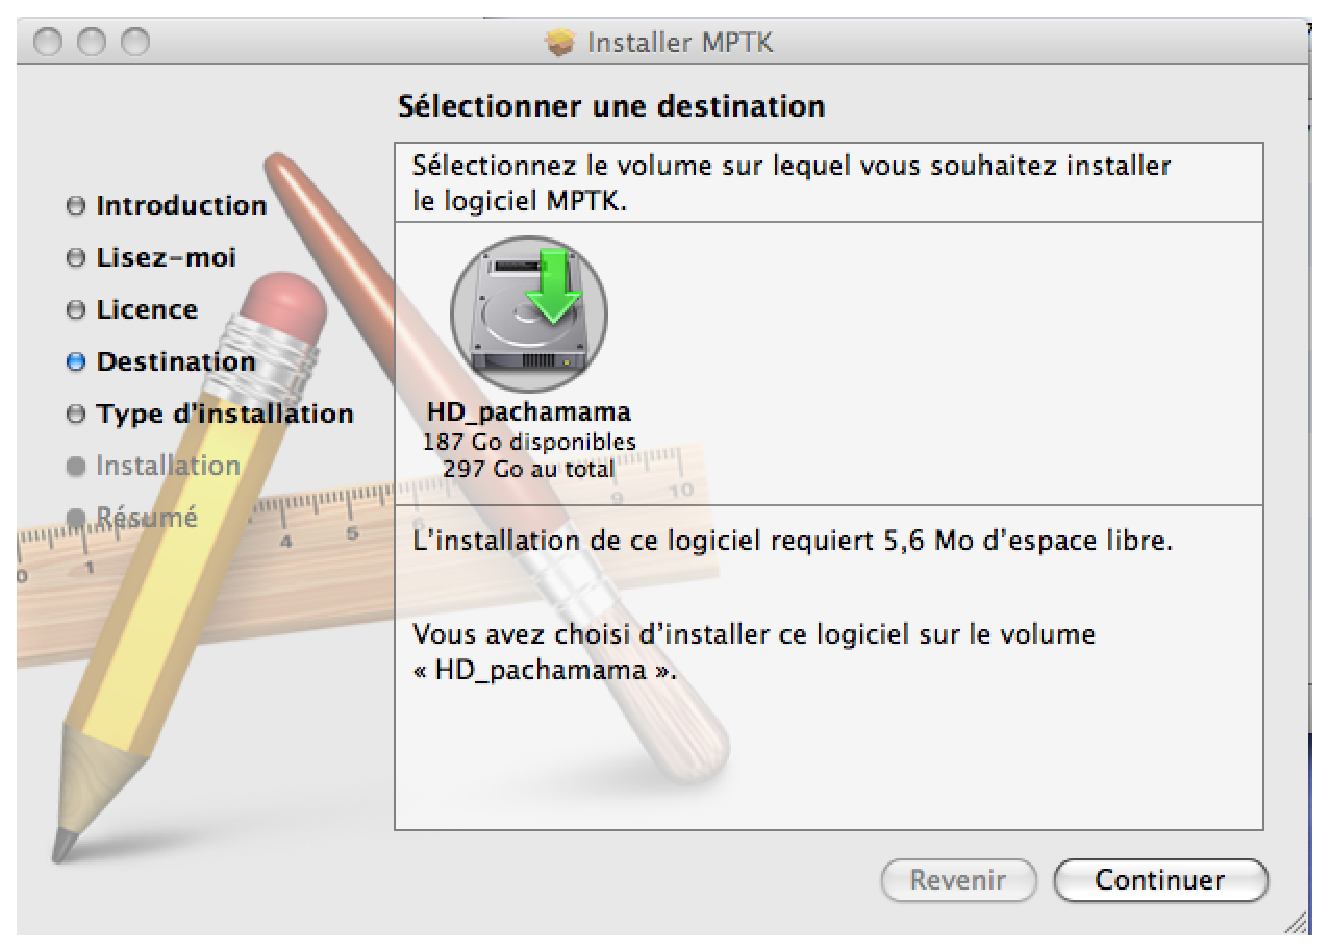
\includegraphics[width = 7cm, height=5cm]{Images/MacPathSelection.eps}
			\textit{\caption{\label{MacPathSelection}Path folder selection}}
		\end{center}
	\end{minipage}
\end{figure}


 %--------------------------------------------------------------
% Section 4.4 : Configuring the path
%--------------------------------------------------------------
\section{Configuring the path}

An environment variable called \begin{footnotesize}MPTK\_CONFIG\_FILENAME\end{footnotesize} needs to be set, 
either temporary, either permanently, with the path of the �path.xml� file located in the \emph{``path\_to\_MPTK/mptk''} directory. 
This file defines the environment paths that MPTK needs to work properly.

% Section 4.4.1 : Configuring the path

\subsection{Temporary path configuration}

Here is the way to temporary configure the \begin{footnotesize}MPTK\_CONFIG\_FILENAME\end{footnotesize} environment variable. 
\textbf{Warning :} This is a temporary setting and it needs to be done at each reset of the computer.

\begin{my_itemize}
	\item \emph{With Bash shell :}
	\begin{my_itemize}
		\item \textcolor[rgb]{0.4,0.4,0.4}{export \begin{footnotesize}MPTK\_CONFIG\_FILENAME\end{footnotesize} =``/usr/local/mptk/path.xml''}
	\end{my_itemize}
	\item \emph{With C-shell :}
	\begin{my_itemize}
		\item \textcolor[rgb]{0.4,0.4,0.4}{setenv \begin{footnotesize}MPTK\_CONFIG\_FILENAME\end{footnotesize} ``/usr/local/mptk/path.xml''}
	\end{my_itemize}
	\item \emph{You can check if the environment variable is correctly set with :}
	\begin{my_itemize}
		\item \textcolor[rgb]{0.4,0.4,0.4}{echo \$\begin{footnotesize}MPTK\_CONFIG\_FILENAME\end{footnotesize}}
	\end{my_itemize}
\end{my_itemize}

% Section 4.4.2 : Permanent path configuration

\subsection{Permanent path configuration}

In order to permanently configure the \begin{footnotesize}MPTK\_CONFIG\_FILENAME\end{footnotesize} environment variable, 
add  the bash shell (or the C-shell) configuration sentence to the ``.bashrc'' (or the ``.cshrc'') file situated under your home directory.

% Section 4.4.2 : Matlab path configuration

\subsection{Matlab path configuration}

When launching Matlab, the user needs to configure Matlab to work with MPTK:
\begin{my_itemize}
	\item Configure the working path either by : 
	\begin{my_itemize}
		\item Selecting the current folder as \textcolor[rgb]{0.4,0.4,0.4}{``/usr/local/mptk/matlab''}
		\item Adding the working path using \textcolor[rgb]{0.4,0.4,0.4}{addpath(``/usr/local/mptk/matlab'')}
	\end{my_itemize}
\end{my_itemize}
